%% This documentation was generated with Faust version 2.37.3
%% Fri Nov 11 20:45:49 2022
%% https://faust.grame.fr

\documentclass{article}

\usepackage[utf8]{inputenc}
\usepackage{graphicx}
\usepackage[usenames]{color}
\usepackage{listings}
\usepackage{supertabular}
\usepackage{amsmath}
\usepackage{latexsym, amssymb}
\usepackage{breqn}

% No indent
\setlength{\parindent}{0pt}

% Make LaTeX output a dot when typing an asterisk
\DeclareMathSymbol{*}{\mathbin}{symbols}{"01}

% lstlistings setup
\definecolor{yobg}{rgb}{0.9,0.9,1}
\definecolor{yotxt}{rgb}{0.01,0.01,0.52} % a dark blue.
\definecolor{mylstbg}{rgb}{0.98,0.98,0.98} % a really pale grey.
\definecolor{mylstcmt}{rgb}{0.01,0.52,0.01} % a dark green.
\definecolor{mylstdoc}{rgb}{0.80,0.30,0.80} % a medium pink.

\lstset{%
  language=C++, 
  numbers=left,%none,
  tabsize=4, 
  frame=single, 
  breaklines=true, 
  numberstyle=\tiny\ttfamily, 
  backgroundcolor=\color{mylstbg}, 
  basicstyle=\scriptsize\ttfamily, 
  commentstyle=\slshape\color{mylstcmt}, %\itshape,
  frameround=tttt, 
  columns=flexible, %fixed, 
  showstringspaces=false,
  emptylines=2,
  inputencoding=utf8,
  extendedchars=true,
  literate=	{á}{{\'a}}1 
			{à}{{\`a}}1 
			{ä}{{\"a}}1 
			{â}{{\^a}}1
			{é}{{\'e}}1 
			{è}{{\`e}}1 
			{ë}{{\"e}}1 
			{ê}{{\^e}}1
			{ï}{{\"i}}1 
			{î}{{\^i}}1
			{ö}{{\"o}}1 
			{ô}{{\^o}}1
			{è}{{\`e}}1 
			{ù}{{\`u}}1 
			{û}{{\^u}}1
			{ç}{{\c{c}}}1 
			{Ç}{{\c{C}}}1,
  emph={component, declare, environment, import, library, process},
  emph={[2]ffunction, fconstant, fvariable},
  emph={[3]button, checkbox, vslider, hslider, nentry, vgroup, hgroup, tgroup, vbargraph, hbargraph, attach},
  emphstyle=\color{yotxt}, %\underline, %\bfseries,
  morecomment=[s][\color{mylstdoc}]{<mdoc>}{</mdoc>},
  rulecolor=\color{black}
}

\newcommand{\faustfilename}{moog.dsp}
\newcommand{\faustdocdir}{moog-mdoc}
\newcommand{\faustprogname}{moog}
\newcommand{\faustversion}{2.37.3}
\newcommand{\faustdocdate}{November 11, 2022}

\begin{document}
\title{moog} \date{\today} \maketitle \begin{tabular}{ll}  \hline  \textbf{compile_options} & -lang cpp -es 1 -single -ftz 0 \\  \textbf{filename} & moog.dsp \\  \textbf{maths.lib/author} & GRAME \\  \textbf{maths.lib/copyright} & GRAME \\  \textbf{maths.lib/license} & LGPL with exception \\  \textbf{maths.lib/name} & Faust Math Library \\  \textbf{maths.lib/version} & 2.5 \\  \textbf{nom} & moog \\  \textbf{platform.lib/name} & Generic Platform Library \\  \textbf{platform.lib/version} & 0.2 \\  \hline \end{tabular} \bigskip  \bigskip Ce document fournit une description mathématique du texte du programme Faust enregistré dans le fichier \texttt{\faustfilename}. Pour davantage d'informations, se reporter à la notice, section\,\ref{notice} (page\,\pageref{notice}).   \section{Définition mathématique de \texttt{process}} \label{equation}  Le programme \emph{\faustprogname} évalue le transformateur de signaux dénoté par \texttt{process}, mathématiquement définit comme suit\,: 
% Ensemble d'équations Faust (correspondant à une balise <equation>).
\begin{enumerate}

\item Signal de sortie $y$ avec
	\begin{dgroup*}
		\begin{dmath*}
				y(t) = p_{8}(t) *  \left(r_{2}(t) - 0.333333333333333 * r_{1}(t)\right) 
		\end{dmath*}
	\end{dgroup*}

\item Signal d'entrée (aucun)

\item Signaux d'interface-utilisateur entrants  ${u_s}_i$ pour $i \in [1,5]$ avec
	\begin{center}
		\begin{supertabular}{lll}
			\textsf{"Frequency"}  & ${u_s}_{1}(t)$ $\in$ $\left[\,50, 5000\,\right]$ & $(\mbox{valeur par défaut} = 150)$\\
			\textsf{"Delta"}  & ${u_s}_{2}(t)$ $\in$ $\left[\,0, 10\,\right]$ & $(\mbox{valeur par défaut} = 1)$\\
			\textsf{"Cutoff"}  & ${u_s}_{3}(t)$ $\in$ $\left[\,100, 5000\,\right]$ & $(\mbox{valeur par défaut} = 600)$\\
			\textsf{"Gain"}  & ${u_s}_{4}(t)$ $\in$ $\left[\,0, 10\,\right]$ & $(\mbox{valeur par défaut} = 0)$\\
			\textsf{"Drive"}  & ${u_s}_{5}(t)$ $\in$ $\left[\,1, 100\,\right]$ & $(\mbox{valeur par défaut} = 1)$\\
		\end{supertabular}
	\end{center}

\item Signaux intermédiaires  $p_i$ pour $i \in [1,8]$,  $s_i$ pour $i \in [1,4]$ et  $r_i$ pour $i \in [1,10]$ avec
	\begin{dgroup*}
		\begin{dmath*}
				p_{1}(t) = k_{2} *  \left({u_s}_{2}(t) + {u_s}_{1}(t)\right) 
		\end{dmath*}
		\begin{dmath*}
				p_{2}(t) = k_{2} * {u_s}_{1}(t)
		\end{dmath*}
		\begin{dmath*}
				p_{3}(t) = {u_s}_{5}(t) * {u_s}_{4}(t)
		\end{dmath*}
		\begin{dmath*}
				p_{4}(t) = k_{3} * p_{3}(t) * {u_s}_{3}(t)
		\end{dmath*}
		\begin{dmath*}
				p_{5}(t) = k_{4} * {u_s}_{3}(t)
		\end{dmath*}
		\begin{dmath*}
				p_{6}(t) = \frac{1}{p_{5}(t) + 1}
		\end{dmath*}
		\begin{dmath*}
				p_{7}(t) = 0.5 * p_{3}(t)
		\end{dmath*}
		\begin{dmath*}
				p_{8}(t) = \frac{1}{{u_s}_{5}(t)}
		\end{dmath*}
	\end{dgroup*}


	\begin{dgroup*}
		\begin{dmath*}
				s_{1}(t) =  \left( \left(r_{7}(t) + -0.5 \hiderel{>} 0\right)  +  \left(r_{6}(t) + -0.5 \hiderel{>} 0\right)  + -1\right) 
		\end{dmath*}
		\begin{dmath*}
				s_{2}(t) = {r_{3}(t)}^{3}
		\end{dmath*}
		\begin{dmath*}
				s_{3}(t) = {r_{4}(t)}^{3}
		\end{dmath*}
		\begin{dmath*}
				s_{4}(t) = {r_{5}(t)}^{3}
		\end{dmath*}
	\end{dgroup*}


	\begin{dgroup*}
		\begin{dmath*}
				r_{6}(t) = p_{1}(t) + r_{6}(t\!-\!1)\pmod{1}
		\end{dmath*}
		\begin{dmath*}
				r_{7}(t) = p_{2}(t) + r_{7}(t\!-\!1)\pmod{1}
		\end{dmath*}
		\begin{dmath*}
				r_{5}(t) = p_{6}(t) *  \left(r_{5}(t\!-\!1) + p_{4}(t) * s_{1}(t)\right) 
		\end{dmath*}
		\begin{dmath*}
				r_{4}(t) = p_{6}(t) *  \left(r_{4}(t\!-\!1) + p_{5}(t) * r_{5}(t)\right) 
		\end{dmath*}
		\begin{dmath*}
				r_{3}(t) = p_{6}(t) *  \left(r_{3}(t\!-\!1) + p_{5}(t) * r_{4}(t)\right) 
		\end{dmath*}
		\begin{dmath*}
				r_{2}(t) = p_{6}(t) *  \left(r_{2}(t\!-\!1) + p_{5}(t) * r_{3}(t)\right) 
		\end{dmath*}
		\begin{dmath*}
				r_{10}(t) = p_{6}(t) *  \left(r_{10}(t\!-\!1) + p_{5}(t) *  \left({p_{7}(t) * s_{1}(t)}^{3} - s_{4}(t)\right) \right) 
		\end{dmath*}
		\begin{dmath*}
				r_{9}(t) = p_{6}(t) *  \left(r_{9}(t\!-\!1) + p_{5}(t) *  \left( \left(s_{4}(t) + r_{10}(t)\right)  - s_{3}(t)\right) \right) 
		\end{dmath*}
		\begin{dmath*}
				r_{8}(t) = p_{6}(t) *  \left(r_{8}(t\!-\!1) + p_{5}(t) *  \left( \left(s_{3}(t) + r_{9}(t)\right)  - s_{2}(t)\right) \right) 
		\end{dmath*}
		\begin{dmath*}
				r_{1}(t) = p_{6}(t) *  \left(r_{1}(t\!-\!1) + p_{5}(t) *  \left( \left(s_{2}(t) + r_{8}(t)\right)  - {r_{2}(t)}^{3}\right) \right) 
		\end{dmath*}
	\end{dgroup*}

\item Constantes $k_i$ pour $i \in [1,4]$ avec
	\begin{dgroup*}
		\begin{dmath*}
				k_{1} = \min\left( 192000, \max\left( 1, f_S \right) \right)
		\end{dmath*}
		\begin{dmath*}
				k_{2} = \frac{1}{k_{1}}
		\end{dmath*}
		\begin{dmath*}
				k_{3} = \frac{\pi}{k_{1}}
		\end{dmath*}
		\begin{dmath*}
				k_{4} = \frac{2*\pi}{k_{1}}
		\end{dmath*}
	\end{dgroup*}

\end{enumerate}

 \section{Bloc-diagramme de \texttt{process}} \label{diagram}  La figure\,\ref{figure1} (page\,\pageref{figure1}) représente le bloc-diagramme de \texttt{process}. \begin{figure}[ht!]
	\centering
	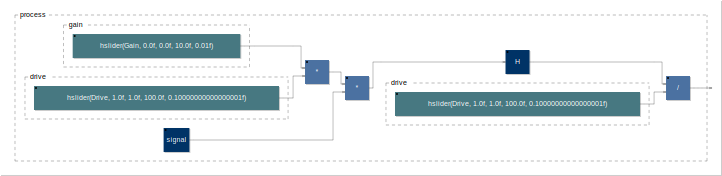
\includegraphics[width=\textwidth]{../svg/svg-01/process}
	\caption{Bloc-diagramme de \texttt{process}}
	\label{figure1}
\end{figure}

 \section{Notice} \label{notice}  
\begin{itemize}
	\item Ce document a été généré par Faust version \faustversion\ (\faustdocdate).
	\item La valeur d'un programme Faust est le résultat de l'application aux signaux d'entrée du transformateur de signaux dénoté par l'expression liée à l'identifiant \texttt{process}. Les signaux sont échantillonnés à la fréquence $f_S$.
	\item Faust (\emph{Functional Audio Stream}) est un langage de programmation fonctionnelle conçu pour des applications synchrones de traitement du signal en temps réel et de synthèse sonore. Un programme Faust est un ensemble de liaisons entre un identifiant et une expression dénotant un transformateur de signaux. Un signal $s$ de $S$ est une fonction\footnote{Faust suppose que $\forall \, s \in S, \forall \, t \in \mathbb{Z}, s(t) = 0 \mathrm{\ quand\ } t < 0$.} du temps $t \in \mathbb{Z}$ vers des valeurs $s(t) \in \mathbb{R}$, tandis qu'un transformateur de signaux est une fonction de $S^n$ vers $S^m$, pour $n,m\in \mathbb{N}$. Se reporter au manuel de Faust pour des informations complémentaires (\textsf{http://faust.grame.fr}).
	\item Dans ce document, les équations mathématiques dérivées d'une expression Faust ont été normalisées par le compilateur Faust (d'une façon dépendante de l'implémentation).
	\item Un bloc-diagramme est une représentation graphique d'une liaison entre un identifiant Faust I et une expression E\,; chaque graphe est placé dans une boîte étiquetée par I. Les sous-expressions de E sont affichées récursivement tant que l'image tient sur une page.
	\item Le répertoire \texttt{\faustdocdir/} peut aussi inclure les répertoires suivants\,:
\begin{itemize}
	\item	\texttt{cpp/} pour le code Faust compilé\,; 
	\item	\texttt{pdf/}, qui contient ce document\,; 
	\item	\texttt{src/} pour toutes les sources Faust utilisées (y compris les bibliothèques)\,; 
	\item	\texttt{svg/} pour les blocs-diagrammes, encodés en SVG (\emph{Scalable Vector Graphics}, \textsf{http://www.w3.org/Graphics/SVG/})\,;
	\item	\texttt{tex/} pour le source \LaTeX\ de ce document.
\end{itemize}
\end{itemize}

 \section{Code Faust} \label{listing}  Cette section contient le code des différents fichiers Faust qui ont été utilisés pour générer ce document. 
\bigskip\bigskip
\begin{lstlisting}[caption=\texttt{moog.dsp}]
import("stdfaust.lib");
// Constants
// Sampling rate
fs = ma.SR;
ts = 1/fs;
// Cutoff frequency
fc = hslider("Cutoff", 600, 100, 5000, 0.1);
// Normalized pulsation
nu = fc*2*ma.PI*ts;

// One-layer filter
// Linear kernel
F1 = *(nu/(1+nu)): +~*(1/(1+nu));
// Third order kernel
t3 = -1/3;
F3 = _<: F1 ,( _ <: (F1 : ^(3) : *(-1)), ^(3) : + : *(t3) : F1) : +;

// module used each time 
M(u1, u3) = F1(u1), F1(u1^3-F1(u1)^3+u3);
M2 = ((_<:(F1, (_^(3), F1^3:>-))), _):_,((_,_):>+:F1);
M3 = (((_<:(((F1<:(_,^(3)))),^(3))):_,((_,_):>-)),_):_,((_,_):>+:F1);
process4 = _,((_,_):>+);

S(u1, u3) = u1 + t3*u3;
S2 = (_,*(t3)):>+;

// four layers filter
H = _,0:M:M:M:M:S;

phaser(f) = ((f/fs):(+:fmod(_,1))~_);

sawtooth(f) = phaser(f) - 0.5;

square(f) = (sawtooth(f) > 0) - 0.5;

drive = hslider("Drive", 1, 1, 100, 0.1);
freq = hslider("Frequency", 150, 50, 5000, 0.1);
delta = hslider("Delta", 1, 0, 10, 0.01);
gain = hslider("Gain", 0, 0, 10, 0.01);

signal = (square(freq)+square(freq+delta)) / 2;

moog = gain * drive * signal: H / drive;

process = moog;
\end{lstlisting}


\bigskip\bigskip
\begin{lstlisting}[caption=\texttt{stdfaust.lib}]
//################################ stdfaust.lib ##########################################
// The purpose of this library is to give access to all the Faust standard libraries
// through a series of environments.
//########################################################################################

aa = library("aanl.lib");
sf = library("all.lib");
an = library("analyzers.lib");
ba = library("basics.lib");
co = library("compressors.lib");
de = library("delays.lib");
dm = library("demos.lib");
dx = library("dx7.lib");
en = library("envelopes.lib");
fd = library("fds.lib");
fi = library("filters.lib");
ho = library("hoa.lib");
it = library("interpolators.lib");
ma = library("maths.lib");
mi = library("mi.lib");
ef = library("misceffects.lib");
os = library("oscillators.lib");
no = library("noises.lib");
pf = library("phaflangers.lib");
pl = library("platform.lib");
pm = library("physmodels.lib");
qu = library("quantizers.lib");
rm = library("reducemaps.lib");
re = library("reverbs.lib");
ro = library("routes.lib");
sp = library("spats.lib");
si = library("signals.lib");
so = library("soundfiles.lib");
sy = library("synths.lib");
ve = library("vaeffects.lib");
vl = library("version.lib");
wa = library("webaudio.lib");
wd = library("wdmodels.lib");
\end{lstlisting}


\bigskip\bigskip
\begin{lstlisting}[caption=\texttt{maths.lib}]
//################################### maths.lib ##########################################
//  Mathematic library for Faust. Its official prefix is `ma`.
//########################################################################################
// Some functions are implemented as Faust foreign functions of `math.h` functions
// that are not part of Faust's primitives. Defines also various constants and several
// utilities.
//########################################################################################

// ## History
// * 06/13/2016 [RM]	normalizing and integrating to new libraries
// * 07/08/2015	[YO]	documentation comments
// * 20/06/2014	[SL]	added FTZ function
// * 22/06/2013	[YO]	added float|double|quad variants of some foreign functions
// * 28/06/2005	[YO]	postfixed functions with 'f' to force float version instead of double
// * 28/06/2005	[YO]	removed 'modf' because it requires a pointer as argument

/************************************************************************
************************************************************************
FAUST library file
Copyright (C) 2003-2016 GRAME, Centre National de Creation Musicale
----------------------------------------------------------------------
This program is free software; you can redistribute it and/or modify
it under the terms of the GNU Lesser General Public License as
published by the Free Software Foundation; either version 2.1 of the
License, or (at your option) any later version.

This program is distributed in the hope that it will be useful,
but WITHOUT ANY WARRANTY; without even the implied warranty of
MERCHANTABILITY or FITNESS FOR A PARTICULAR PURPOSE.  See the
GNU Lesser General Public License for more details.

You should have received a copy of the GNU Lesser General Public
License along with the GNU C Library; if not, write to the Free
Software Foundation, Inc., 59 Temple Place, Suite 330, Boston, MA
02111-1307 USA.

EXCEPTION TO THE LGPL LICENSE : As a special exception, you may create a
larger FAUST program which directly or indirectly imports this library
file and still distribute the compiled code generated by the FAUST
compiler, or a modified version of this compiled code, under your own
copyright and license. This EXCEPTION TO THE LGPL LICENSE explicitly
grants you the right to freely choose the license for the resulting
compiled code. In particular the resulting compiled code has no obligation
to be LGPL or GPL. For example you are free to choose a commercial or
closed source license or any other license if you decide so.
************************************************************************
************************************************************************/

// This library contains platform specific constants 
pl = library("platform.lib");
ma = library("maths.lib"); // for compatible copy/paste out of this file

declare name "Faust Math Library";
declare version "2.5";
declare author "GRAME";
declare copyright "GRAME";
declare license "LGPL with exception";

//=============================Functions Reference========================================
//========================================================================================


//---------------------------------`(ma.)SR`---------------------------------------
// Current sampling rate. Constant during
// program execution.
//
// #### Usage
//
// ```
// SR : _
// ```
//-----------------------------------------------------------------------------
SR = pl.SR;


//---------------------------------`(ma.)BS`---------------------------------------
// Current block-size. Can change during the execution.
//
// #### Usage
//
// ```
// BS : _
// ```
//-----------------------------------------------------------------------------
BS = pl.BS;


//---------------------------------`(ma.)PI`---------------------------------------
// Constant PI in double precision.
//
// #### Usage
//
// ```
// PI : _
// ```
//-----------------------------------------------------------------------------
PI = 3.14159265358979323846;


//---------------------------------`(ma.)E`---------------------------------------
// Constant e in double precision.
//
// #### Usage
//
// ```
// E : _
// ```
//-----------------------------------------------------------------------------
E = 2.71828182845904523536;


//---------------------------------`(ma.)EPSILON`---------------------------------------
// Constant EPSILON in simple/double/quad precision.
//
// #### Usage
//
// ```
// EPSILON : _
// ```
//-----------------------------------------------------------------------------
singleprecision EPSILON = 1.192092896e-07;
doubleprecision EPSILON = 2.2204460492503131e-016;
quadprecision EPSILON = 2.2204460492503131e-016;
fixedpointprecision EPSILON = 2.2204460492503131e-016;


//---------------------------------`(ma.)MIN`---------------------------------------
// Constant MIN in simple/double/quad precision (minimal positive value).
//
// #### Usage
//
// ```
// MIN : _
// ```
//-----------------------------------------------------------------------------
singleprecision MIN = 1.175494351e-38;
doubleprecision MIN = 2.2250738585072014e-308;
quadprecision MIN = 2.2250738585072014e-308;
fixedpointprecision MIN = 2.2250738585072014e-308;


//---------------------------------`(ma.)MAX`------------------------------
// Constant MAX in simple/double/quad precision (maximal positive value).
//
// #### Usage
//
// ```
// MAX : _
// ```
//-----------------------------------------------------------------------------
singleprecision MAX = 3.402823466e+38;
doubleprecision MAX = 1.7976931348623158e+308;
quadprecision MAX = 1.7976931348623158e+308;
fixedpointprecision MAX = 1.7976931348623158e+308;

// Obsolete, kept for compatibility reasons
INFINITY = MAX; 

//---------------------------------`(ma.)FTZ`---------------------------------------
// Flush to zero: force samples under the "maximum subnormal number"
// to be zero. Usually not needed in C++ because the architecture
// file take care of this, but can be useful in JavaScript for instance.
//
// #### Usage
//
// ```
// _ : FTZ : _
// ```
//
// #### Reference
//
// <http://docs.oracle.com/cd/E19957-01/806-3568/ncg_math.html>
//-----------------------------------------------------------------------------
FTZ(x) = x * (abs(x) > MIN);


//---------------------------------`(ma.)copysign`---------------------------------------
// Changes the sign of x (first input) to that of y (second input).
//
// #### Usage
//
// ```
// _,_ : copysign : _
// ```
//-----------------------------------------------------------------------------
copysign = ffunction(float copysignf|copysign|copysignl (float, float), <math.h>,"");


//---------------------------------`(ma.)neg`---------------------------------------
// Invert the sign (-x) of a signal.
//
// #### Usage
//
// ```
// _ : neg : _
// ```
//-----------------------------------------------------------------------------
neg(x) = -x;


//-------`(ma.)sub(x,y)`------------------
// Subtract `x` and `y`.
//
// #### Usage
//
// ```
// _,_ : sub : _
// ```
//------------------------------
sub(x,y) = y-x;


//---------------------------------`(ma.)inv`---------------------------------------
// Compute the inverse (1/x) of the input signal.
//
// #### Usage
//
// ```
// _ : inv : _
// ```
//-----------------------------------------------------------------------------
inv(x) = 1/x;


//---------------------------------`(ma.)cbrt`--------------------------------------
// Computes the cube root of of the input signal.
//
// #### Usage
//
// ```
// _ : cbrt : _
// ```
//-----------------------------------------------------------------------------
cbrt = ffunction(float cbrtf|cbrt|cbrtl (float), <math.h>,"");


//---------------------------------`(ma.)hypot`-------------------------------------
// Computes the euclidian distance of the two input signals
// sqrt(x*x+y*y) without undue overflow or underflow.
//
// #### Usage
//
// ```
// _,_ : hypot : _
// ```
//-----------------------------------------------------------------------------
hypot = ffunction(float hypotf|hypot|hypotl (float, float), <math.h>,"");


//---------------------------------`(ma.)ldexp`-------------------------------------
// Takes two input signals: x and n, and multiplies x by 2 to the power n.
//
// #### Usage
//
// ```
// _,_ : ldexp : _
// ```
//-----------------------------------------------------------------------------
ldexp = ffunction(float ldexpf|ldexp|ldexpl (float, int), <math.h>,"");


//---------------------------------`(ma.)scalb`-------------------------------------
// Takes two input signals: x and n, and multiplies x by 2 to the power n.
//
// #### Usage
//
// ```
// _,_ : scalb : _
// ```
//-----------------------------------------------------------------------------
scalb = ffunction(float scalbnf|scalbn|scalbnl (float, int), <math.h>,"");


//---------------------------------`(ma.)log1p`----------------------------------
// Computes log(1 + x) without undue loss of accuracy when x is nearly zero.
//
// #### Usage
//
// ```
// _ : log1p : _
// ```
//-----------------------------------------------------------------------------
log1p = ffunction(float log1pf|log1p|log1pl (float), <math.h>,"");


//---------------------------------`(ma.)logb`---------------------------------------
// Return exponent of the input signal as a floating-point number.
//
// #### Usage
//
// ```
// _ : logb : _
// ```
//-----------------------------------------------------------------------------
logb = ffunction(float logbf|logb|logbl (float), <math.h>,"");


//---------------------------------`(ma.)ilogb`-------------------------------------
// Return exponent of the input signal as an integer number.
//
// #### Usage
//
// ```
// _ : ilogb : _
// ```
//-----------------------------------------------------------------------------
ilogb = ffunction(int ilogbf|ilogb|ilogbl (float), <math.h>,"");


//---------------------------------`(ma.)log2`-------------------------------------
// Returns the base 2 logarithm of x.
//
// #### Usage
//
// ```
// _ : log2 : _
// ```
//-----------------------------------------------------------------------------
log2(x) = log(x)/log(2.0);


//---------------------------------`(ma.)expm1`-------------------------------------
// Return exponent of the input signal minus 1 with better precision.
//
// #### Usage
//
// ```
// _ : expm1 : _
// ```
//-----------------------------------------------------------------------------
expm1 = ffunction(float expm1f|expm1|expm1l (float), <math.h>,"");


//---------------------------------`(ma.)acosh`-------------------------------------
// Computes the principle value of the inverse hyperbolic cosine
// of the input signal.
//
// #### Usage
//
// ```
// _ : acosh : _
// ```
//-----------------------------------------------------------------------------
acosh = ffunction(float acoshf|acosh|acoshl (float), <math.h>, "");


//--------------------------------`(ma.)asinh`-----------------------------------
// Computes the inverse hyperbolic sine of the input signal.
//
// #### Usage
//
// ```
// _ : asinh : _
// ```
//-----------------------------------------------------------------------------
asinh = ffunction(float asinhf|asinh|asinhl (float), <math.h>, "");


//--------------------------------`(ma.)atanh`-----------------------------------
// Computes the inverse hyperbolic tangent of the input signal.
//
// #### Usage
//
// ```
// _ : atanh : _
// ```
//-----------------------------------------------------------------------------
atanh = ffunction(float atanhf|atanh|atanhl (float), <math.h>, "");


//---------------------------------`(ma.)sinh`---------------------------------------
// Computes the hyperbolic sine of the input signal.
//
// #### Usage
//
// ```
// _ : sinh : _
// ```
//-----------------------------------------------------------------------------
sinh = ffunction(float sinhf|sinh|sinhl (float), <math.h>, "");


//---------------------------------`(ma.)cosh`--------------------------------------
// Computes the hyperbolic cosine of the input signal.
//
// #### Usage
//
// ```
// _ : cosh : _
// ```
//-----------------------------------------------------------------------------
cosh = ffunction(float coshf|cosh|coshl (float), <math.h>, "");


//---------------------------------`(ma.)tanh`--------------------------------------
// Computes the hyperbolic tangent of the input signal.
//
// #### Usage
//
// ```
// _ : tanh : _
// ```
//-----------------------------------------------------------------------------
tanh = ffunction(float tanhf|tanh|tanhl (float), <math.h>,"");


//---------------------------------`(ma.)erf`---------------------------------------
// Computes the error function of the input signal.
//
// #### Usage
//
// ```
// _ : erf : _
// ```
//-----------------------------------------------------------------------------
erf = ffunction(float erff|erf|erfl(float), <math.h>,"");


//---------------------------------`(ma.)erfc`---------------------------------------
// Computes the complementary error function of the input signal.
//
// #### Usage
//
// ```
// _ : erfc : _
// ```
//-----------------------------------------------------------------------------
erfc = ffunction(float erfcf|erfc|erfcl(float), <math.h>,"");


//---------------------------------`(ma.)gamma`-------------------------------------
// Computes the gamma function of the input signal.
//
// #### Usage
//
// ```
// _ : gamma : _
// ```
//-----------------------------------------------------------------------------
gamma = ffunction(float tgammaf|tgamma|tgammal(float), <math.h>,"");


//---------------------------------`(ma.)lgamma`------------------------------------
// Calculates the natural logorithm of the absolute value of
// the gamma function of the input signal.
//
// #### Usage
//
// ```
// _ : lgamma : _
// ```
//-----------------------------------------------------------------------------
lgamma = ffunction(float lgammaf|lgamma|lgammal(float), <math.h>,"");


//----------------------------------`(ma.)J0`---------------------------------------
// Computes the Bessel function of the first kind of order 0
// of the input signal.
//
// #### Usage
//
// ```
// _ : J0 : _
// ```
//-----------------------------------------------------------------------------
J0 = ffunction(float j0(float), <math.h>,"");


//----------------------------------`(ma.)J1`---------------------------------------
// Computes the Bessel function of the first kind of order 1
// of the input signal.
//
// #### Usage
//
// ```
// _ : J1 : _
// ```
//-----------------------------------------------------------------------------
J1 = ffunction(float j1(float), <math.h>,"");


//----------------------------------`(ma.)Jn`---------------------------------------
// Computes the Bessel function of the first kind of order n
// (first input signal) of the second input signal.
//
// #### Usage
//
// ```
// _,_ : Jn : _
// ```
//-----------------------------------------------------------------------------
Jn = ffunction(float jn(int, float), <math.h>,"");


//----------------------------------`(ma.)Y0`---------------------------------------
// Computes the linearly independent Bessel function of the second kind
// of order 0 of the input signal.
//
// #### Usage
//
// ```
// _ : Y0 : _
// ```
//-----------------------------------------------------------------------------
Y0 = ffunction(float y0(float), <math.h>,"");


//----------------------------------`(ma.)Y1`---------------------------------------
// Computes the linearly independent Bessel function of the second kind
// of order 1 of the input signal.
//
// #### Usage
//
// ```
// _ : Y0 : _
// ```
//-----------------------------------------------------------------------------
Y1 = ffunction(float y1(float), <math.h>,"");


//----------------------------------`(ma.)Yn`---------------------------------------
// Computes the linearly independent Bessel function of the second kind
// of order n (first input signal) of the second input signal.
//
// #### Usage
//
// ```
// _,_ : Yn : _
// ```
//-----------------------------------------------------------------------------
Yn = ffunction(float yn(int, float), <math.h>,"");


//----------------------------`(ma.)fabs`, `(ma.)fmax`, `(ma.)fmin`---------------------------
// Just for compatibility...
//
// ```
// fabs = abs
// fmax = max
// fmin = min
// ```
//-----------------------------------------------------------------------------
fabs = abs;
fmax = max;
fmin = min;

//-------------------------------`(ma.)np2`--------------------------------------
// Gives the next power of 2 of x.
//
// #### Usage
//
// ```
// np2(n) : _
// ```
//
// Where:
//
// * `n`: an integer
//-----------------------------------------------------------------------------
np2 = -(1) <: >>(1)|_ <: >>(2)|_ <: >>(4)|_ <: >>(8)|_ <: >>(16)|_ : +(1);


//-----------------------------`(ma.)frac`---------------------------------------
// Gives the fractional part of n.
//
// #### Usage
//
// ```
// frac(n) : _
// ```
//
// Where:
//
// * `n`: a decimal number
//------------------------------------------------------------------------------
frac(n) = n - floor(n);
decimal = frac;
// NOTE: decimal does the same thing as frac but using floor instead. JOS uses frac a lot
// in filters.lib so we decided to keep that one... decimal is declared though for
// backward compatibility.
// decimal(n) = n - floor(n);


//-------------------------------`(ma.)modulo`---------------------------------------
// Modulus operation.
//
// #### Usage
//
// ```
// modulo(x,N) : _
// ```
//
// Where:
//
// * `x`: the numerator
// * `N`: the denominator
//------------------------------------------------------------------------------
modulo(x,N) = (x % N + N) % N;


//---------------`(ma.)isnan`----------------
// Return non-zero if x is a NaN.
//
// #### Usage
//
// ```
// isnan(x)
// _ : isnan : _
// ```
//
// Where:
//
// * `x`: signal to analyse
//------------------------------------------
isnan = ffunction(int isnanf|isnan|isnanl (float),<math.h>,"");


//---------------`(ma.)isinf`----------------
// Return non-zero if x is a positive or negative infinity.
//
// #### Usage
//
// ```
// isinf(x)
// _ : isinf : _
// ```
//
// Where:
//
// * `x`: signal to analyse
//------------------------------------------
isinf = ffunction(int isinff|isinf|isinfl (float),<math.h>,"");

nextafter = ffunction(float nextafter(float, float),<math.h>,"");


//---------------------------`(ma.)chebychev`-------------------------------
// Chebychev transformation of order n.
//
// #### Usage
//
// ```
// _ : chebychev(n) : _
// ```
//
// Where:
//
// * `n`: the order of the polynomial
//
// #### Semantics
//
// ```
// T[0](x) = 1,
// T[1](x) = x,
// T[n](x) = 2x*T[n-1](x) - T[n-2](x)
// ```
//
// #### Reference
//
// <http://en.wikipedia.org/wiki/Chebyshev_polynomial>
//-------------------------------------------------------------------------
chebychev(0,x) = 1;
chebychev(1,x) = x;
chebychev(n,x) = 2*x*chebychev(n-1, x) - chebychev(n-2, x);


//------------------------`(ma.)chebychevpoly`-------------------------------
// Linear combination of the first Chebyshev polynomials.
//
// #### Usage
//
// ```
// _ : chebychevpoly((c0,c1,...,cn)) : _
// ```
//
// Where:
//
// * `cn`: the different Chebychevs polynomials such that:
// 	chebychevpoly((c0,c1,...,cn)) = Sum of chebychev(i)*ci
//
// #### Reference
//
// <http://www.csounds.com/manual/html/chebyshevpoly.html>
//-------------------------------------------------------------------------
chebychevpoly(lcoef) = _ <: L(0,lcoef) :> _
	with {
		L(n,(c,cs)) = chebychev(n)*c, L(n+1,cs);
		L(n,c)      = chebychev(n)*c;
	};


//------------------`(ma.)diffn`----------------------------
// Negated first-order difference.
//
// #### Usage
//
// ```
// _ : diffn : _
// ```
//--------------------------------------------------------
diffn(x) = x' - x; // negated first-order difference


//------------------`(ma.)signum`----------------------------
// The signum function signum(x) is defined as
// -1 for x<0, 0 for x==0, and 1 for x>0.
//
// #### Usage
//
// ```
// _ : signum : _
// ```
//--------------------------------------------------------
signum(x) = (x>0)-(x<0);


//------------------`(ma.)nextpow2`----------------------------
// The nextpow2(x) returns the lowest integer m such that
// 2^m >= x.
//
// #### Usage
//
// ```
// 2^nextpow2(n)
// ```
// Useful for allocating delay lines, e.g., 
// ```
// delay(2^nextpow2(maxDelayNeeded), currentDelay);
// ```
//--------------------------------------------------------
nextpow2(x) = ceil(log(x)/log(2.0));


//--------------------`(ma.)zc`------------------------------------------------
// Indicator function for zero-crossing: it returns 1 if a zero-crossing
// occurs, 0 otherwise.
//
// #### Usage
//
// ```
// _ : zc : _
// ```
//-----------------------------------------------------------------------------
zc(x) = x * x' < 0;

\end{lstlisting}


\bigskip\bigskip
\begin{lstlisting}[caption=\texttt{platform.lib}]
//#################################### platform.lib ########################################
// A library to handle platform specific code in Faust. Its official prefix is `pl`.
//########################################################################################
// It can be reimplemented to globally change the SR and the tablesize definitions


/************************************************************************
************************************************************************
FAUST library file
Copyright (C) 2020 GRAME, Centre National de Creation Musicale
----------------------------------------------------------------------
This program is free software; you can redistribute it and/or modify
it under the terms of the GNU Lesser General Public License as
published by the Free Software Foundation; either version 2.1 of the
License, or (at your option) any later version.

This program is distributed in the hope that it will be useful,
but WITHOUT ANY WARRANTY; without even the implied warranty of
MERCHANTABILITY or FITNESS FOR A PARTICULAR PURPOSE.  See the
GNU Lesser General Public License for more details.

You should have received a copy of the GNU Lesser General Public
License along with the GNU C Library; if not, write to the Free
Software Foundation, Inc., 59 Temple Place, Suite 330, Boston, MA
02111-1307 USA.

EXCEPTION TO THE LGPL LICENSE : As a special exception, you may create a
larger FAUST program which directly or indirectly imports this library
file and still distribute the compiled code generated by the FAUST
compiler, or a modified version of this compiled code, under your own
copyright and license. This EXCEPTION TO THE LGPL LICENSE explicitly
grants you the right to freely choose the license for the resulting
compiled code. In particular the resulting compiled code has no obligation
to be LGPL or GPL. For example you are free to choose a commercial or
closed source license or any other license if you decide so.
************************************************************************
************************************************************************/

declare name "Generic Platform Library";
declare version "0.2";

//---------------------------------`(pl.)SR`-----------------------------------
// Current sampling rate (between 1Hz and 192000Hz). Constant during
// program execution.
//-----------------------------------------------------------------------------
SR = min(192000.0, max(1.0, fconstant(int fSamplingFreq, <math.h>)));

//---------------------------------`(pl.)BS`---------------------------------------
// Current block-size. Can change during the execution.
//-----------------------------------------------------------------------------
BS = fvariable(int count, <math.h>);

//---------------------------------`(pl.)tablesize`----------------------------
// Oscillator table size
//-----------------------------------------------------------------------------
tablesize = 1 << 16;
\end{lstlisting}


\end{document}

